\documentclass{article}
\usepackage[utf8]{inputenc}
\usepackage{hyperref}
\usepackage[letterpaper, portrait, margin=1in]{geometry}
\usepackage{enumitem}
\usepackage{amsmath}
\usepackage{booktabs}
\usepackage{graphicx}

\usepackage{hyperref}
\hypersetup{
colorlinks=true,
    linkcolor=black,
    filecolor=black,      
    urlcolor=blue,
    citecolor=black,
}
\usepackage{natbib}

\usepackage{titlesec}

\title{Homework 6}
\author{Roshani Bulkunde}
\date{February 2023}

\begin{document}

\maketitle

\section{Python}

\subsection{Question 1}
My intuition says it should be Sharp RD. Because the vehicles with the length greater than 225 inches are required to be in the program and you can not manipulate the length of the vehicles. So, there will be full compliance. 

However, fuel efficiency is inversely proportional with length of the vehicle. That makes it fuzzy RD.
 

\subsection{Question 2}
Figure \ref{fig:discontinuity_2} shows a scatter plot with mpg on the y-axis and length − cutoff on the x-axis with a line at the RD cutoff. There is not visual evidence of bunching near the cut-off because the scatter points is distributed all over the graph. It is hard to tell from the figure if there is visual evidence of a discontinuity.

\begin{figure}[ht]
    \centering
    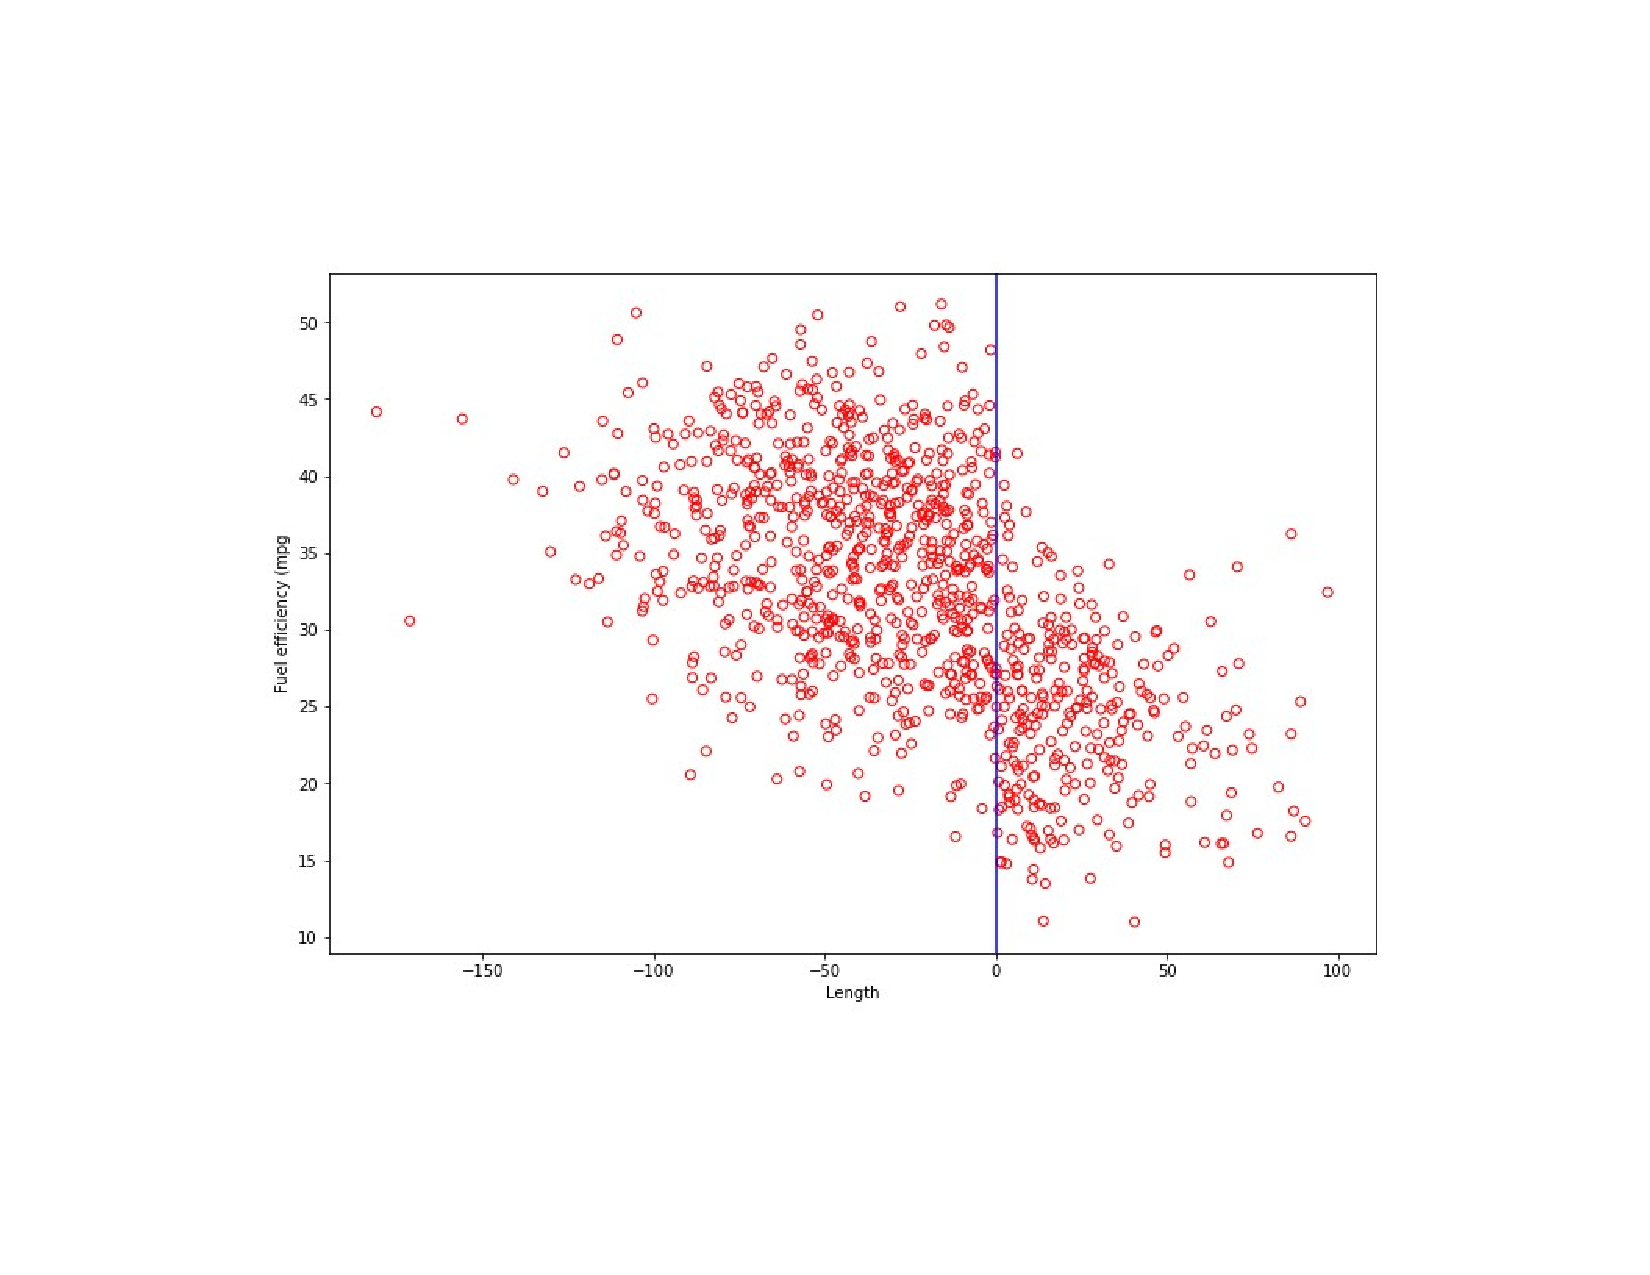
\includegraphics[scale = 0.7]{discontinuity_2.pdf}
    \caption{Plot of a scatterplot}
    \label{fig:discontinuity_2}
\end{figure}


\newpage

\subsection{Question 3 }

Table \ref{tab:RD3_python} first-stage treatment effect estimate after fitting a first-order polynomial to both sides of the cutoff in a regression discontinuity design. The fuel efficiency decrease by 8.27 miles per gallon around the cutoff as the impact of the policy.
\begin{table}[ht]
    \centering
    \begin{tabular}{ll}
\toprule
{} &       0 \\
\midrule
Treated      &   -8.27 \\
             &  (0.65) \\
length       &   -0.04 \\
             &  (0.01) \\
Constant     &   42.12 \\
             &  (1.26) \\
Observations &  1000.0 \\
\bottomrule
\end{tabular}

    \caption{The first-stage treatment effect estimate: fitting the first-order polynomial to both sides of the cutoff in a regression discontinuity design}
    \label{tab:RD3_python}
\end{table}

Figure \ref{fig:discontinuity_3} and \ref{fig:discontinuity_31}  plots the resulting polynomial over a scatterplot.

\newpage

\begin{figure}[ht]
    \centering
    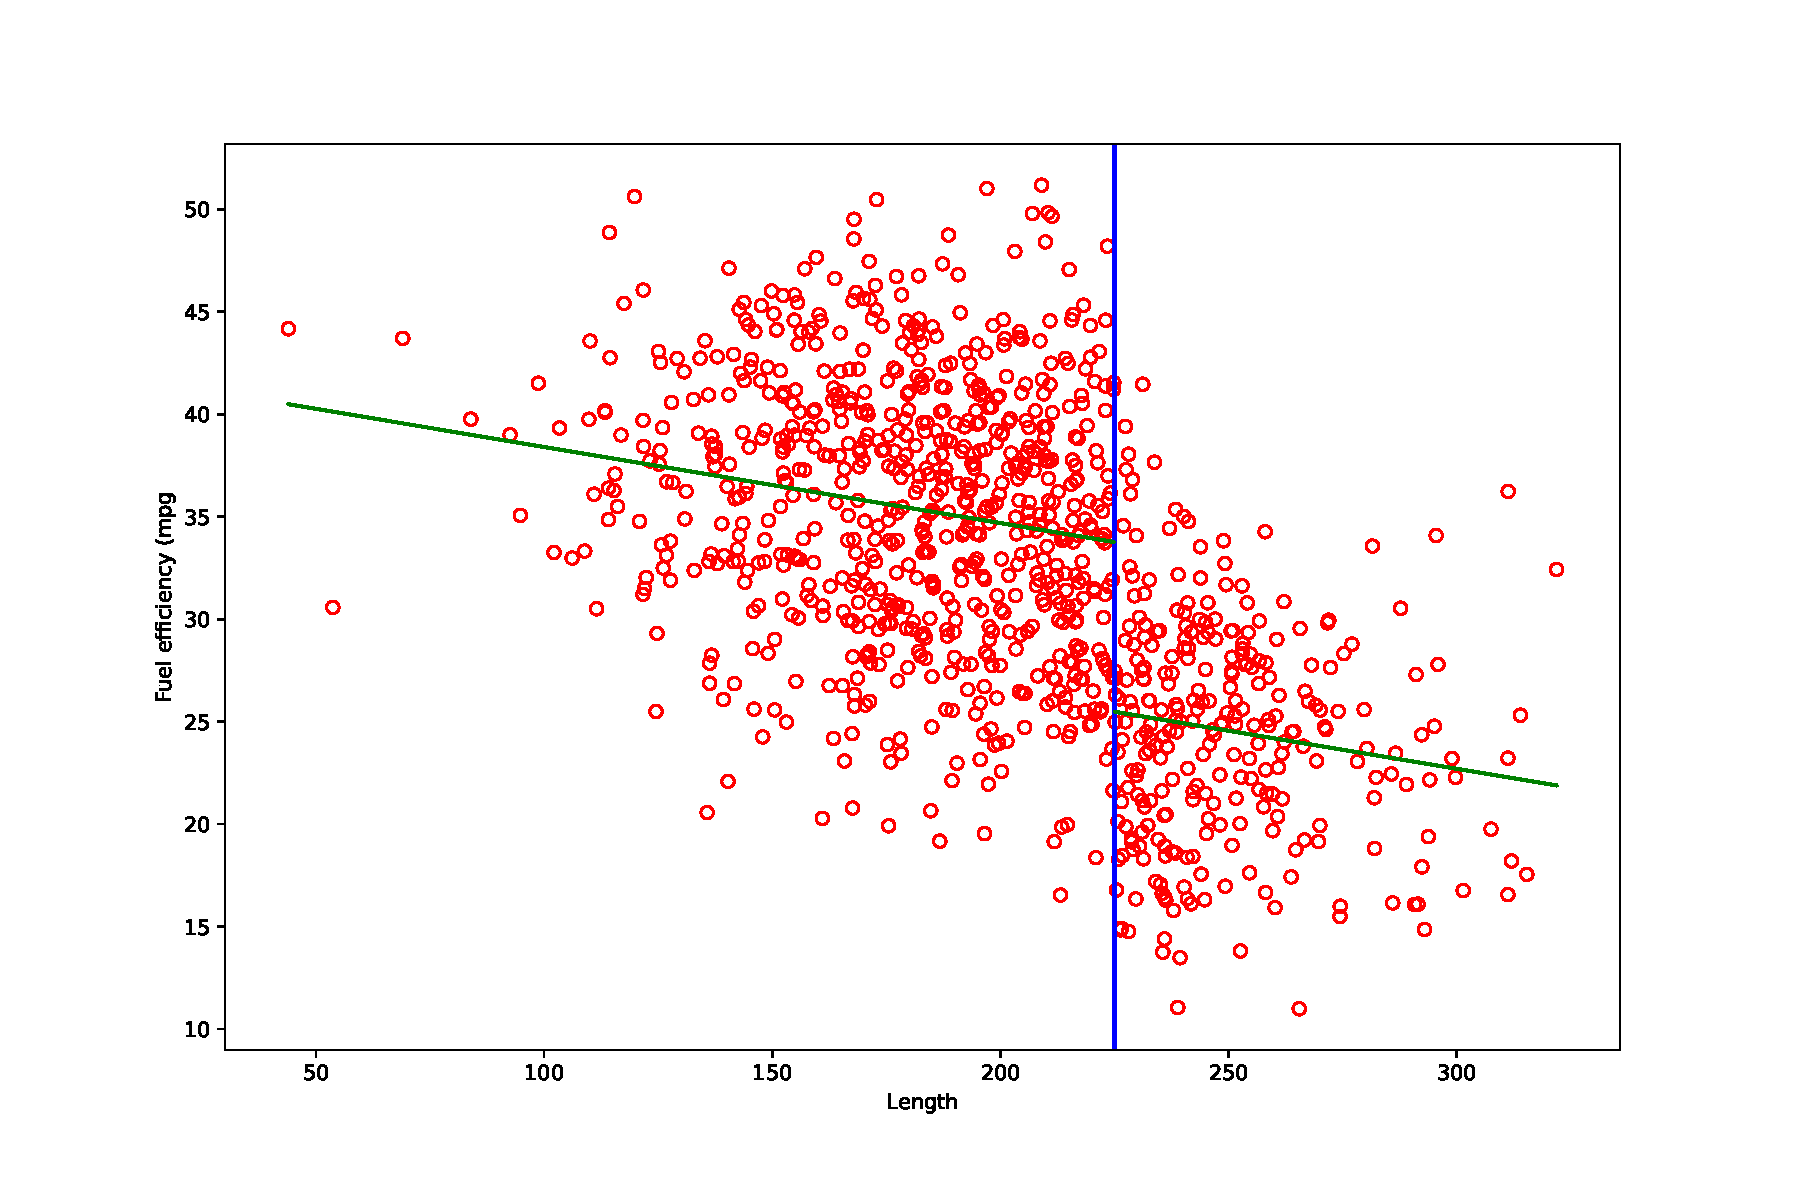
\includegraphics[scale = 0.6]{discontinuity_3.pdf}
    \caption{Plot of the resulting polynomial over a scatterplot: fitting the first-order polynomial to both sides of the cutoff in a regression discontinuity design}
    \label{fig:discontinuity_3}
\end{figure}


\begin{figure}[ht]
    \centering
    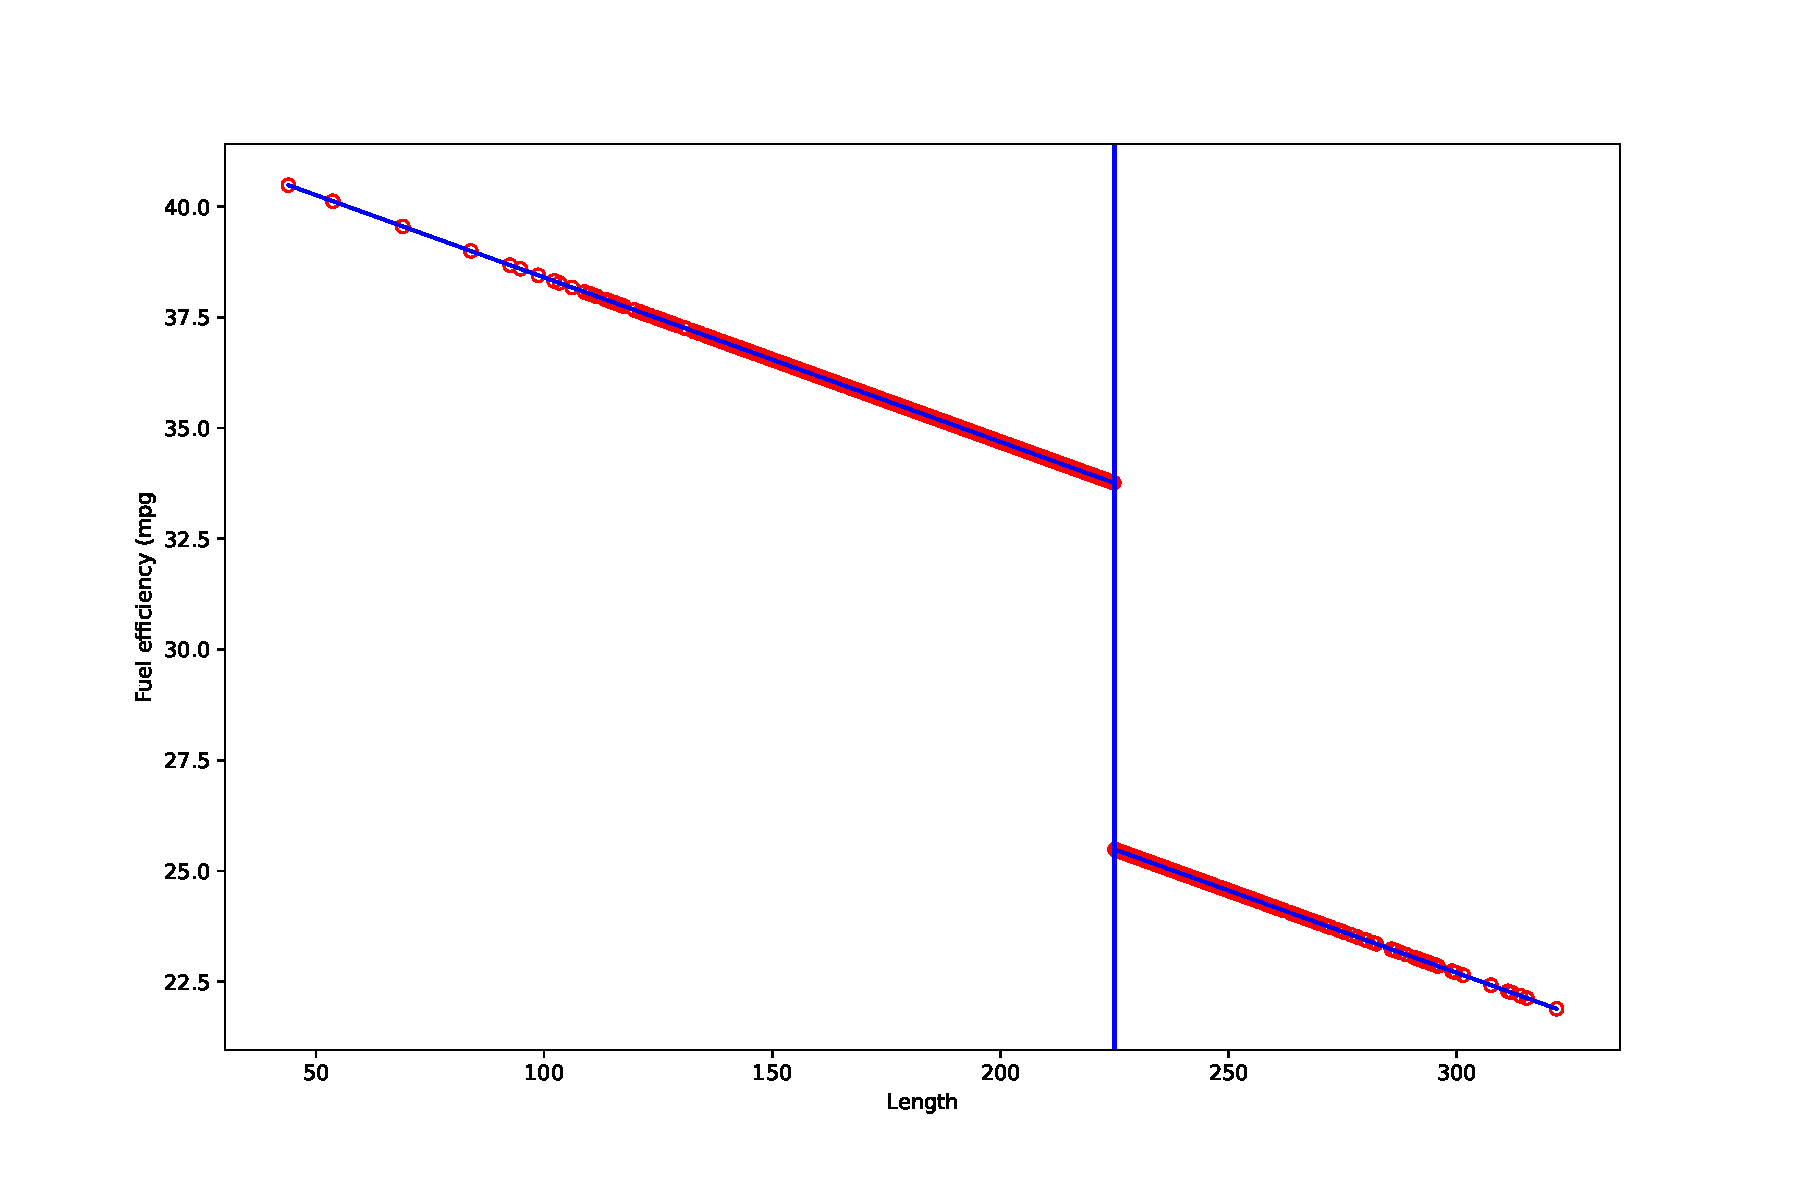
\includegraphics[scale = 0.6]{discontinuity_31.pdf}
    \caption{Plot of the resulting polynomial over a scatterplot}
    \label{fig:discontinuity_31}
\end{figure}

\newpage

\subsection{Question 4 }

\begin{table}[ht]
    \centering
    \begin{tabular}{ll}
\toprule
{} &       0 \\
\midrule
Treated      &   -8.00 \\
             &  (0.70) \\
length       &   -0.00 \\
             &  (0.00) \\
Constant     &   38.66 \\
             &  (0.65) \\
Observations &  1000.0 \\
\bottomrule
\end{tabular}

    \caption{The first-stage treatment effect estimate:fitting a second-order polynomial to both sides of the cutoff in a regression discontinuity design}
    \label{tab:RD4_python}
\end{table}

Table \ref{tab:RD4_python} first-stage treatment effect estimate after fitting a second-order polynomial to both sides of the cutoff in a regression discontinuity design. The fuel efficiency decrease by 8 miles per gallon around the cutoff as the impact of the policy.

Figure \ref{fig:discontinuity_4}  plots the resulting polynomial over a scatterplot.

\begin{figure}[ht]
    \centering
    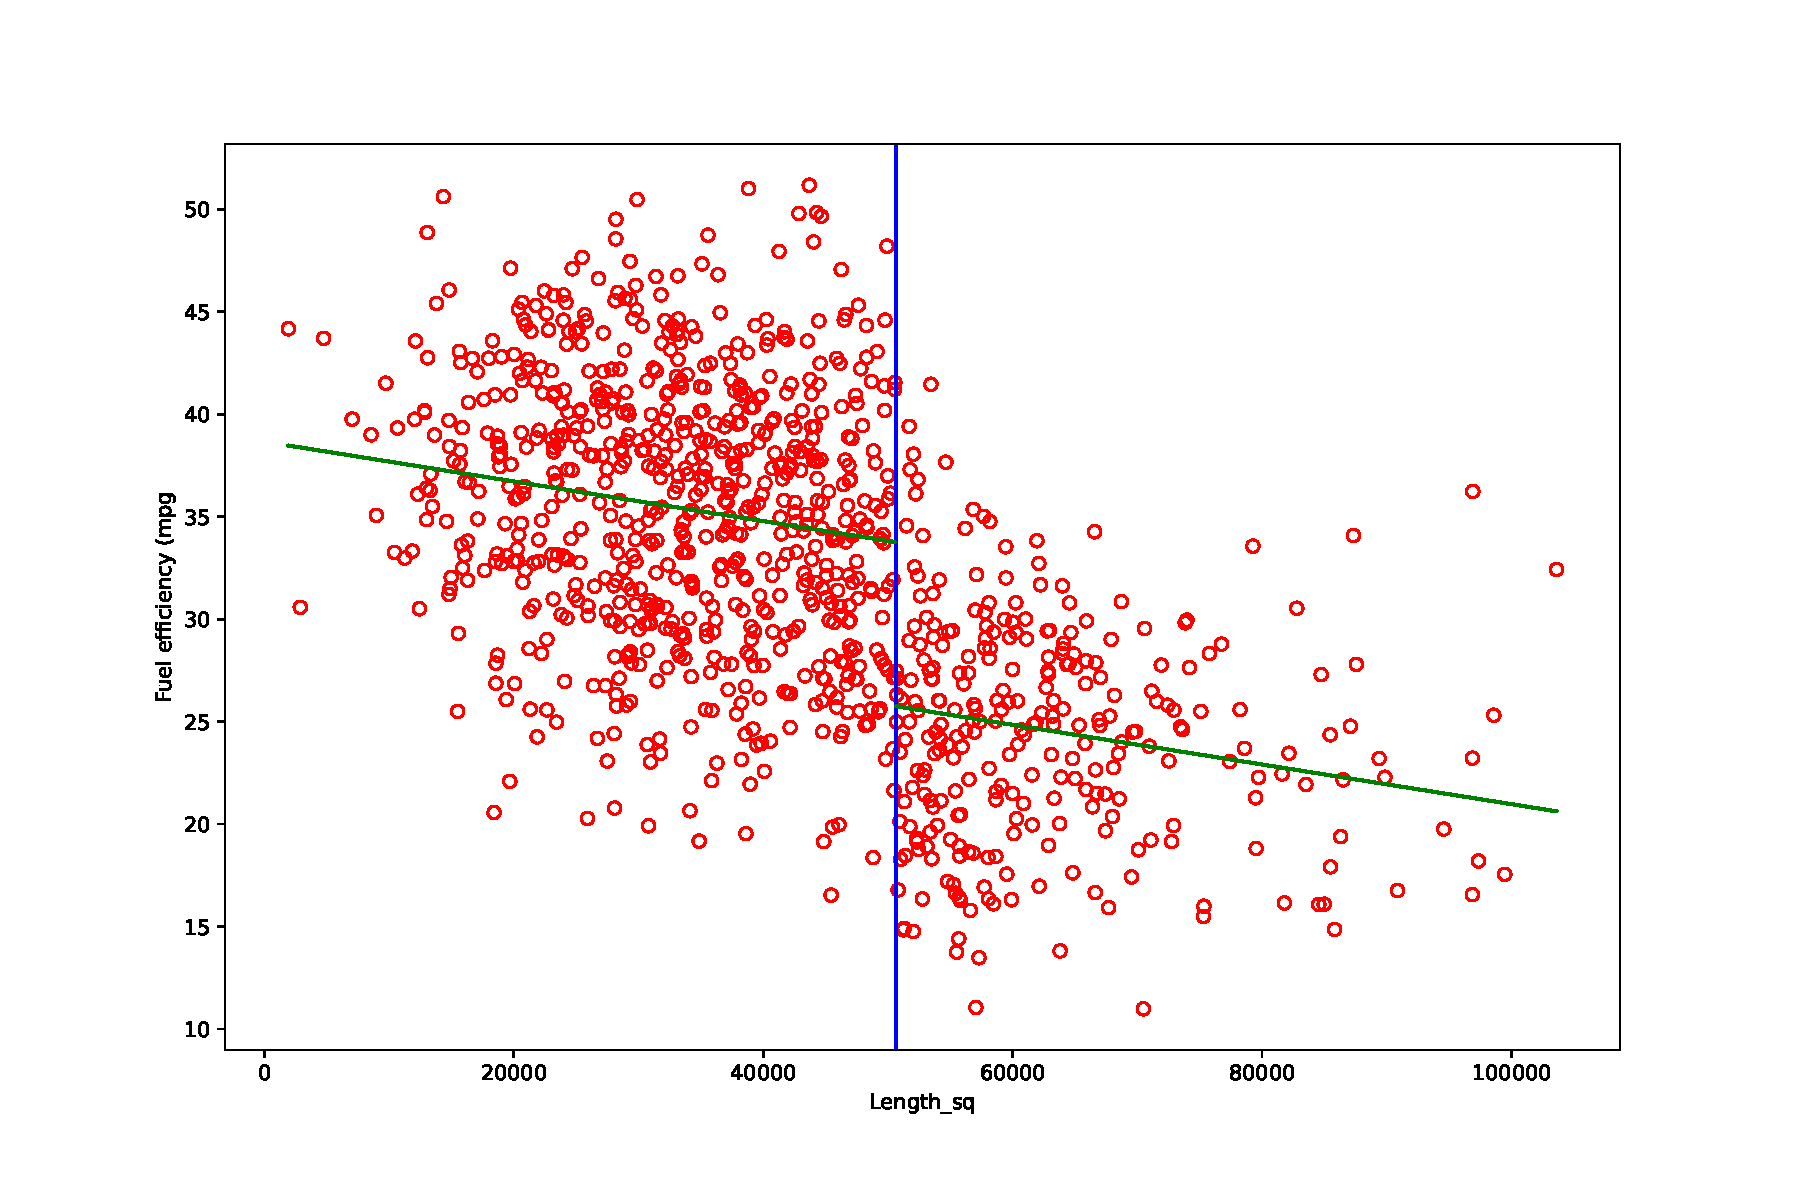
\includegraphics[scale = 0.6]{discontinuity_4.pdf}
    \caption{Plot of the resulting polynomial over a scatterplot: fitting a second-order polynomial to both sides of the cutoff in a regression discontinuity design}
    \label{fig:discontinuity_4}
\end{figure}




\newpage

\subsection{Question 5 }



Table \ref{tab:RD5_python} first-stage treatment effect estimate after fitting a fifth-order polynomial to both sides of the cutoff in a regression discontinuity design. The fuel efficiency decrease by 9 miles per gallon around the cutoff as the impact of the policy.

\begin{table}[ht]
    \centering
    \begin{tabular}{ll}
\toprule
{} &       0 \\
\midrule
Treated      &   -9.02 \\
             &  (0.68) \\
length       &   -0.00 \\
             &  (0.00) \\
Constant     &   35.98 \\
             &  (0.28) \\
Observations &  1000.0 \\
\bottomrule
\end{tabular}

    \caption{The first-stage treatment effect estimate: fitting a fifth-order polynomial to both sides of the cutoff in a regression discontinuity design}
    \label{tab:RD5_python}
\end{table}

\begin{figure}[ht]
    \centering
    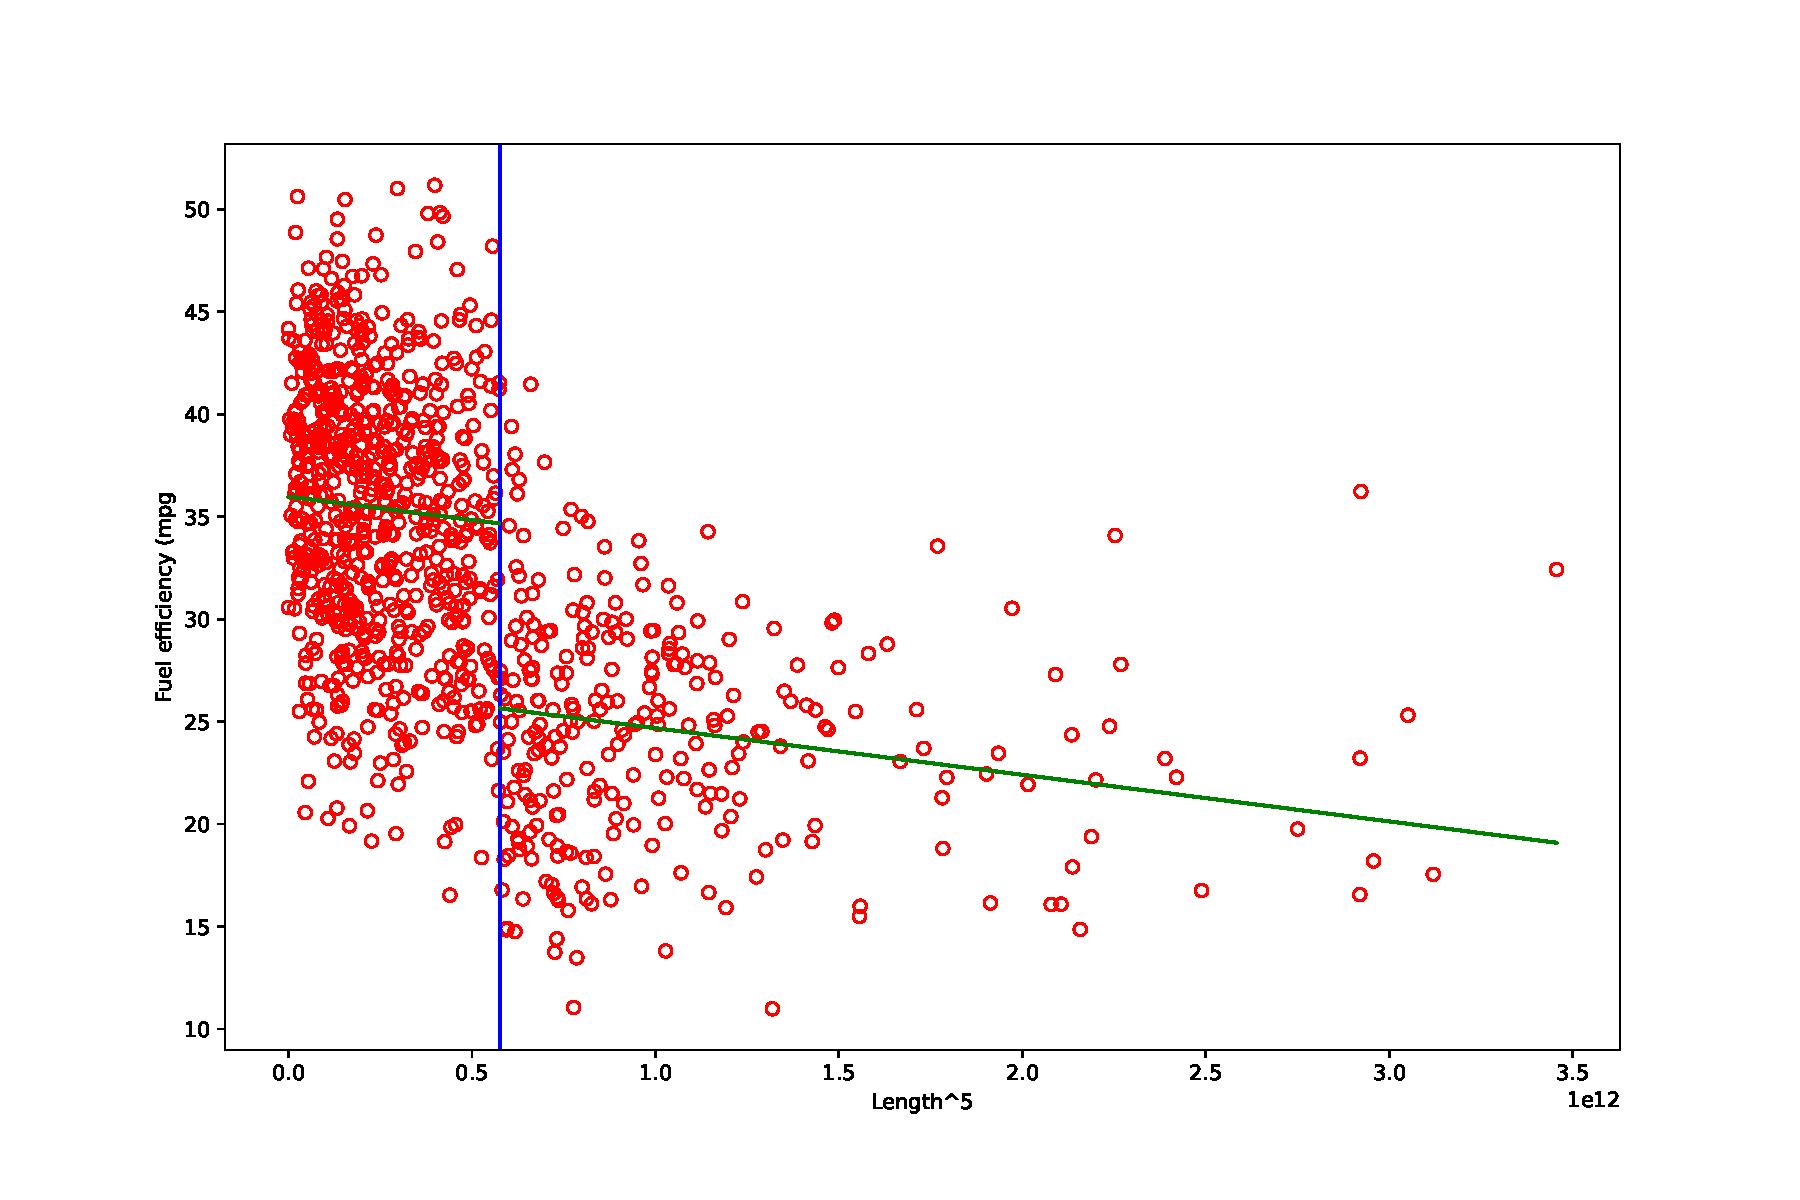
\includegraphics[scale = 0.6]{discontinuity_5.pdf}
    \caption{Plot of the resulting polynomial over a scatterplot: fitting a fifth-order polynomial to both sides of the cutoff in a regression discontinuity design}
    \label{fig:discontinuity_5}
\end{figure}

\newpage

\subsection{Question 6 }
I am using the first-degree polynomial fit for the first stage because from visual representation of scatter plot and the fitted line, I think the first-degree polynomial fit is the best.
\begin{table}[ht]
    \centering
    \begin{tabular}{ll}
\toprule
{} &         0 \\
\midrule
Fuel Efficiency (mpg) &    135.92 \\
                      &   (22.22) \\
Car                   &  -3692.55 \\
                      &  (222.28) \\
Constant              &  17606.11 \\
                      &  (711.95) \\
Observations          &    1000.0 \\
\bottomrule
\end{tabular}

    \caption{The average treatment effect from the second stage}
    \label{tab:RD6_python}
\end{table}

\newpage

\section{STATA}
\subsection{Question 1 }
\subsubsection{Question 1 (a) }

\begin{table}[ht]
    \centering
    \begin{tabular}{lc} \hline
 & (1) \\
VARIABLES & Price (USD) \\ \hline
 &  \\
Fuel Efficiency (mpg) & 158.3*** \\
 & (29.55) \\
Car & -4,743*** \\
 & (355.8) \\
Constant & 17,407*** \\
 & (848.2) \\
 &  \\
Observations & 1,000 \\
 R-squared & 0.096 \\ \hline
\multicolumn{2}{c}{ Robust standard errors in parentheses} \\
\multicolumn{2}{c}{ *** p$<$0.01, ** p$<$0.05, * p$<$0.1} \\
\end{tabular}

    \caption{The average treatment effect from the second stage}
    \label{tab:Rd_2sls_stata}
\end{table}

\newpage

\subsubsection{Question 1 (b) }

\begin{figure}[ht]
    \centering
    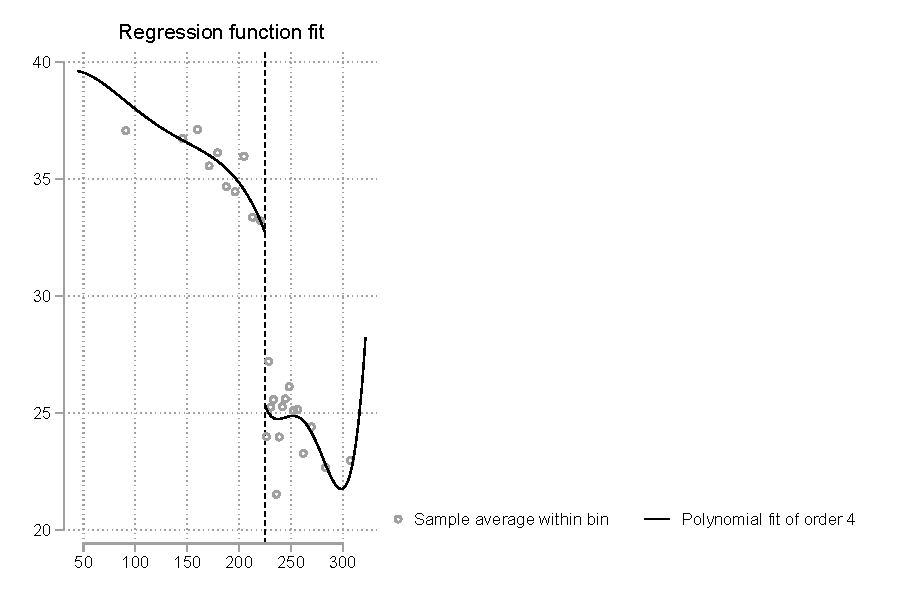
\includegraphics[scale = 0.7]{rdplot_stata.pdf}
    \caption{a plot of the results using rdplot}
    \label{fig:rdplot_stata}
\end{figure}

\newpage

\subsection{Question 2 }
I think discontinuity is the valid instrument. Length of the vehicle is as good as random, and installing the new technology depends on the length of the vehicle. Discontinuity will impact on hedonic price only through the mpg. 

\end{document}
